\chapter{Simulated Annealing}

\section{Theoretical Foundations}

\textit{Simulated annealing (SA)} is a probabilistic technique for approximating the global optimum of a given function, often used when the search space is discrete.
The name of the algorithm comes from annealing in metallurgy, a technique involving heating and controlled cooling of a material to alter its physical properties.
Simulated annealing can be used for very hard computational optimization problems where exact algorithms fail; even though it usually achieves an approximate solution to the global minimum, it could be enough for many practical problems.
This notion of \textbf{slow, controlled cooling} implemented in the simulated annealing algorithm \textbf{is interpreted as a slow decrease in the probability of accepting worse solutions} as the solution space is explored. Accepting worse solutions allows for a more extensive search for the global optimal solution, because it allows to overcome the characteristic shortcoming of simple hill-climbing algorithms, that is, being very prone to find local minima.

\subsection{Fundamental Concepts}\label{ann_fund_concepts}

In general, simulated annealing algorithms work as follows. The temperature progressively decreases from an initial positive value to zero. At each time step, the algorithm randomly selects a solution close to the current one, measures its quality, and moves to it according to the temperature-dependent probabilities of selecting better or worse solutions, which during the search respectively remain at 1 (or positive) and decrease towards zero.
\par
Each fundamental concept of the Simulated Annealing approach is better described in the following paragraphs.

\paragraph{Energy Function} Energy is defined as a function that assigns a score to some provided state of the system. The better the state, that is, the closer such a state is to the solution of the problem, the lower the score assigned to it. Therefore, minimizing the energy function means trying to find a solution to the problem at hand. 

\paragraph{The basic iteration} At each step, the simulated annealing heuristic considers some neighboring state $s^\star$ of the current state $s$, and probabilistically decides between moving the system to state $s^\star$ or staying in the current state $s$. These probabilities ultimately lead the system to move to states of lower energy. Typically, this step is repeated until the system reaches a state that is good enough for the application, or until a given computation budget has been exhausted.

\paragraph{Neighbouring States} The neighbours of a state of the problem are defined as states produced by applying minimal alterations to the former. Such states are evaluated when trying to optimize the solution in an attempt to progressively improve the current state.

\paragraph{Acceptance Probabilities}  The probability of making the transition from the current state $s$ to a candidate new state $s_{new}$ is specified by an acceptance function $P(e, e_{new}, T)$, that depends on the energies $e$ and $e_{new}$ of the two states, and on a global time-varying parameter $T$ called temperature.
It is recalled that states with a smaller energy are better than those with a greater energy. Therefore, in order to prevent the method from becoming stuck at a local minimum that is worse than the global one, the probability function $P$ must be positive even when  $e_{new}$ is greater than $e$. However, when $T$ tends to zero, the probability $P(e, e_{new}, T)$ must tend to zero if $e_{new} > e$ and to a positive value otherwise. For sufficiently small values of $T$, the system will then increasingly favor moves that go \textit{downhill} (i.e., to lower energy values), and avoid those that go \textit{uphill}. With $T = 0$ the procedure reduces to the greedy algorithm, which makes only the downhill transitions.
\par
A commonly used acceptance probability function with the above characteristics is defined as

$$
P(e, e_{new}, T) = \left\{
    \begin{array}{ll}
          1, \text{ if } e < e_{new} \\
          P[X \leq \exp({\frac{-(e_{new} - e)}{T}})] \text{ otherwise} \\
    \end{array} 
\right.
$$

where $X$ is a random variable that follows a uniform distribution in the closed interval $[0, 1]$.

\subsection{Theory Applied to the Sudoku Problem}

The solution of the Sudoku problem is a grid that completes the partially initialized, starting one, with 1 to 9 digits, in such a way that there are no repetitions of numbers in every row, column and box. For this reason, the energy function can be defined as one that penalizes states with a higher number of repetitions across the three Sudoku "dimensions" (col, row, box), i.e. states with a higher number of repetitions have a higher energy. Additionally, in Sudoku, a neighbouring state can be thought of as a Sudoku grid that differs from the original state by just a handful of cells, possibly just one or two.
Finally, the probability acceptance function can be the commonly used one defined in the previous section.

\section{Software Implementation}

The core parts of the implementation are the main function, which implements the simulated annealing process, state representation and the way neighbors are generated, the energy function, the acceptance probability function and the temperature reset process in case the solver is stuck on a local minimum.

\subsection{Fundamental Data Structures}

The majority of the fundamental data structures used to implement this approach are the same ones described at section \ref{cp_data_structs}. More specifically, \textit{SudokuGrid} serves as the supertype of the class \textit{SimulatedAnnealingGrid}, which basically represents the state of the system. As such, it provides an interface to easily calculate its energy and to generate a neighbouring state, i.e. perform the so called \textit{move} action.

\subsection{Main Function and General Intuition}\label{sim_ann_main_func}

The general intuition behind the procedure used to find the Sudoku solution is that, at each iteration of the algorithm (referred to as \textit{epoch}), the next (neighboring) state is obtained by swapping two cells of a same, random, row, and this is repeated until a solution is found or some computational budget is exceeded. During the initialization phase, in fact, the starting grid was filled in such a way that each row contained exactly one occurrence of every Sudoku number (from 1 to 9). This approach allowed to reformulate the problem into finding the correct set of row permutations such that all the Sudoku constraints are respected.
\par
Below is an image of the main part of the aforementioned Simulated Annealing loop.

\begin{figure}[h]
    \centering
    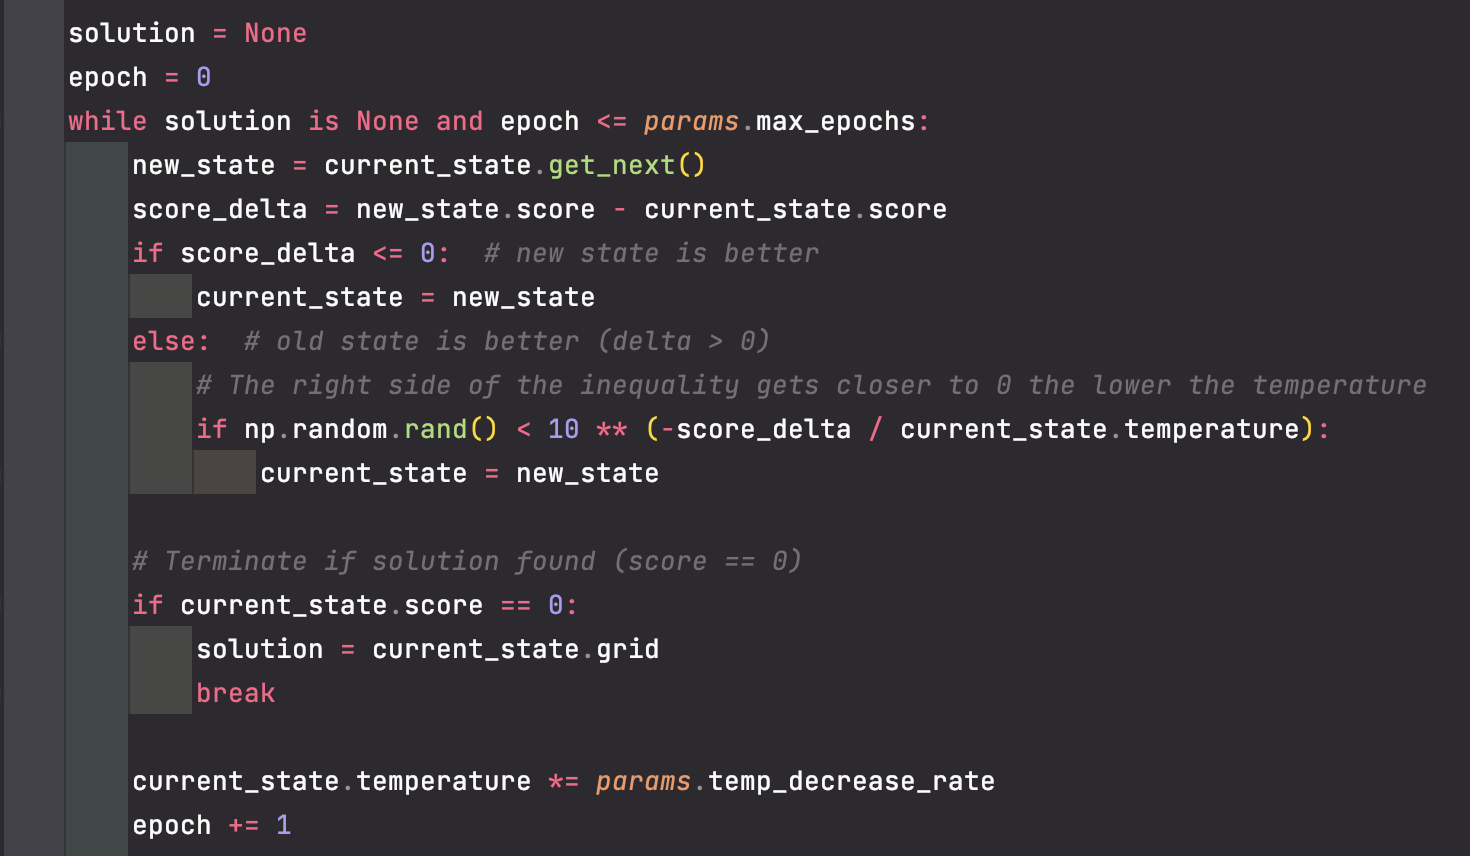
\includegraphics[scale=0.65]{assignment-1/images/sim_ann/main-2-body.png}
    \caption{Main Simulated Annealing loop}
    \label{fig:ann_main_1}
\end{figure}

\par
Another important part of the development of the solver was to introduce a \textit{temperature reset step} in case the algorithm stayed "stuck" for too long. This, along with the parameters of the solver and a brief parenthesis on the acceptance probability function, are better discussed in the following subsections.

\subsubsection{Parameters}

The solver accepts the three main parameters shown, along with their respective descriptions, in the below image. The initial values assigned to these parameters were empirically determined:

\begin{itemize}
    \item a \textit{starting temperature} of $3$, which is a value close to that of $T$ such that $\log_{10}{-\Delta{E} / T} = 0.7$, with $ExpectedValue(\Delta{E}) \sim 2$; in other words, the starting temperature was chosen so that the probability of accepting a worse state at the beginning was close to 70\%

    \item a \textit{temperature decrease rate} of $0.95$, with the goal of decreasing the temperature relatively fast, albeit not too much; this was to compensate for the temperature reset step, that periodically raised the temperature to a relatively high level

    \item a \textit{computational budget}, represented by the $max\_epochs$ parameter, big enough to allow to solve even relatively hard Sudoku grids; the value of such a parameter was set to $3*10^6$
\end{itemize}

\begin{figure}[h]
    \centering
    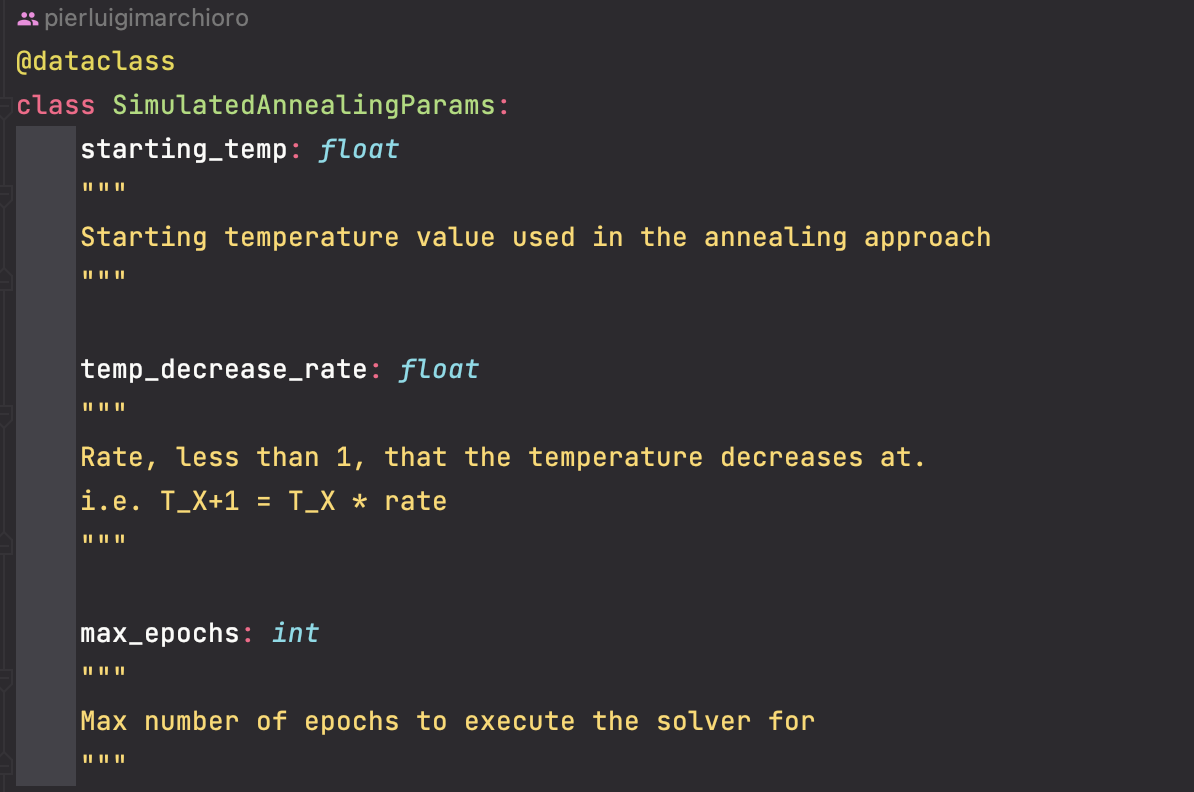
\includegraphics[scale=0.65]{assignment-1/images/sim_ann/main-1-params.png}
    \caption{Parameters of the Simulated Annealing procedure}
    \label{fig:ann_main_2_params}
\end{figure}

\subsubsection{Acceptance Probability Function}

The implementation of such a function can be seen at image \ref{fig:ann_main_1}, and it refers to the "canonical" acceptance probability function described at section \ref{ann_fund_concepts}.

\subsubsection{Temperature Reset}

As mentioned before, in order to allow the algorithm to "recover" in case it was "stuck", a temperature reset step was implemented. \textit{Being stuck} means that the score of the state chosen at each iteration didn't vary for more than $stuckness\_threshold$ times, with $stuckness\_threshold$ being set to $100$. For each iteration at and after such a threshold was reached, the formula in the following image was applied to obtain the new temperature level:

\begin{figure}[h]
    \centering
    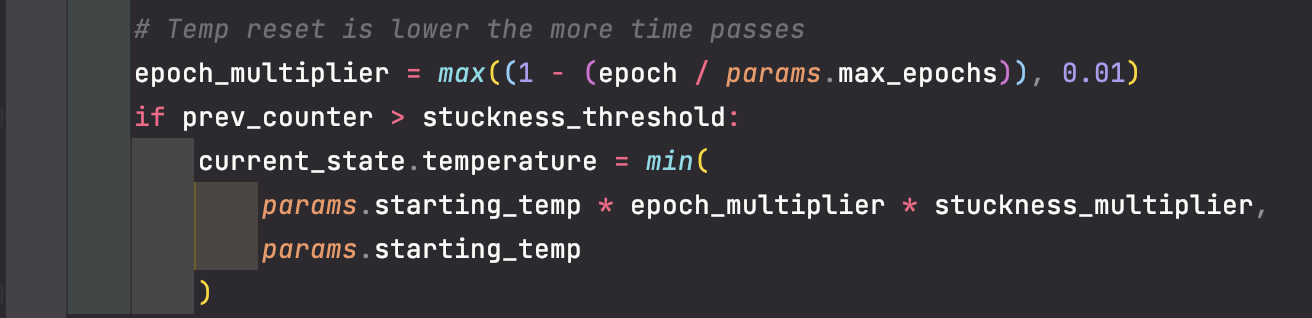
\includegraphics[scale=0.65]{assignment-1/images/sim_ann/main-3-temp-reset.png}
    \caption{Temperature Reset Formula}
    \label{fig:ann_main_3_temp_reset}
\end{figure}

It is noted that the new temperature reset level is a function of the \textit{starting temperature}, as well as of two other parameters:

\begin{itemize}
    \item $stuckness\_multiplier$, which increases the more the algorithm is stuck on a certain score
    \item $epoch\_multiplier$, which decreases the more the computational budget of the algorithm is exhausted (i.e. time passes); additionally, this parameter was capped at $0.01$ so that the probability of accepting a worse state would never become too low
\end{itemize}

\subsection{State Representation and Neighbor Generation}

State representation and neighbor generation were both mainly handled by the \textit{SimulatedAnnealingState} class, which provided as a useful wrapper for a, previously described, \textit{SimulatedAnnealingGrid} instance. The goal of such a class was to provide a simple interface to perform the \textit{move} action, implemented by the \textit{get\_next()} method, and the calculation of the energy of some grid state, referred to as \textit{score}. 
\par
The below images show how such an interface and such actions were implemented.

\begin{figure}[h]
    \centering
    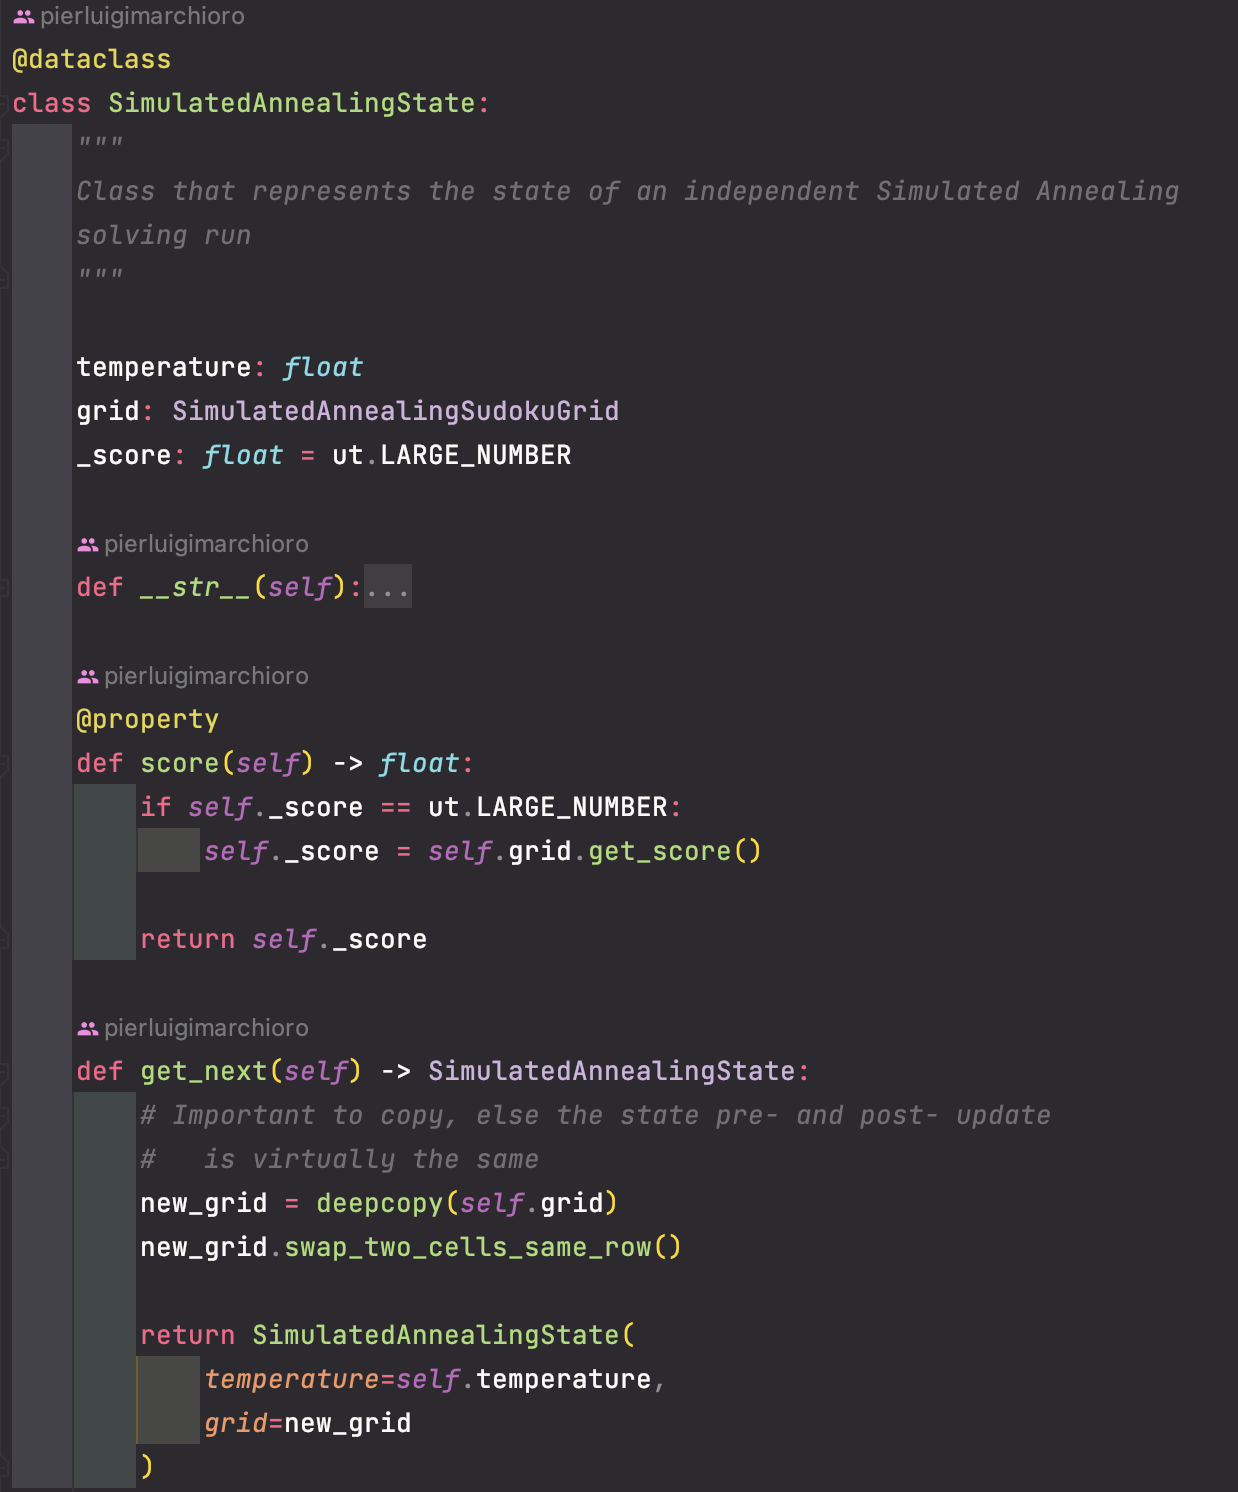
\includegraphics[scale=0.5]{assignment-1/images/sim_ann/neighbors-1-sim_ann_state.png}
    \caption{\textit{SimulatedAnnealingState} class}
    \label{fig:ann_state_1}
\end{figure}

\begin{figure}[h]
    \centering
    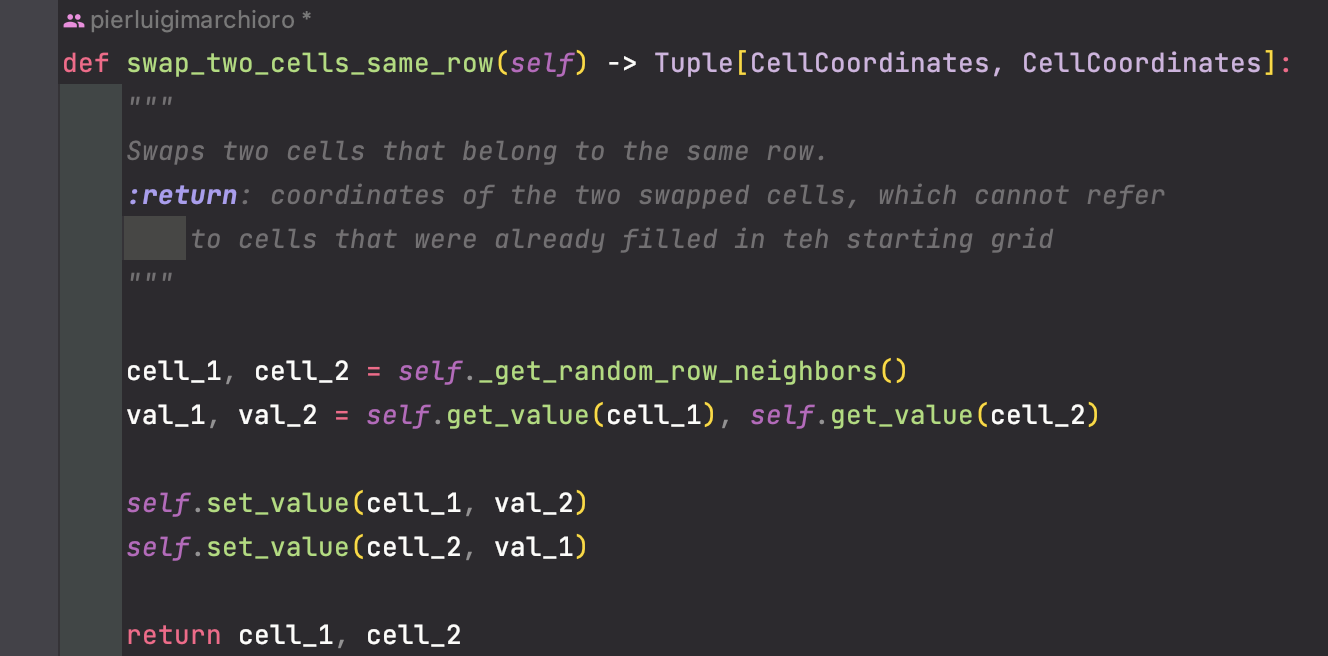
\includegraphics[scale=0.65]{assignment-1/images/sim_ann/neighbors-2-swap.png}
    \caption{Implementation of the \textit{move} action - Two random cells of the same random row are swapped}
    \label{fig:ann_state_2_swap}
\end{figure}


\subsection{Energy Function}

As hinted to before, this is referred to, in the solver implementation, as \textit{scoring function}. Such a function was defined so that the score associated to a Sudoku grid was the sum of the duplicates in each of its columns and boxes. Rows were not counted, because, as previously discussed at \ref{sim_ann_main_func}, the solver maintains the invariant that each row always contains exactly one occurrence of each Sudoku number, therefore never presenting any duplicate.

\begin{figure}[h]
    \centering
    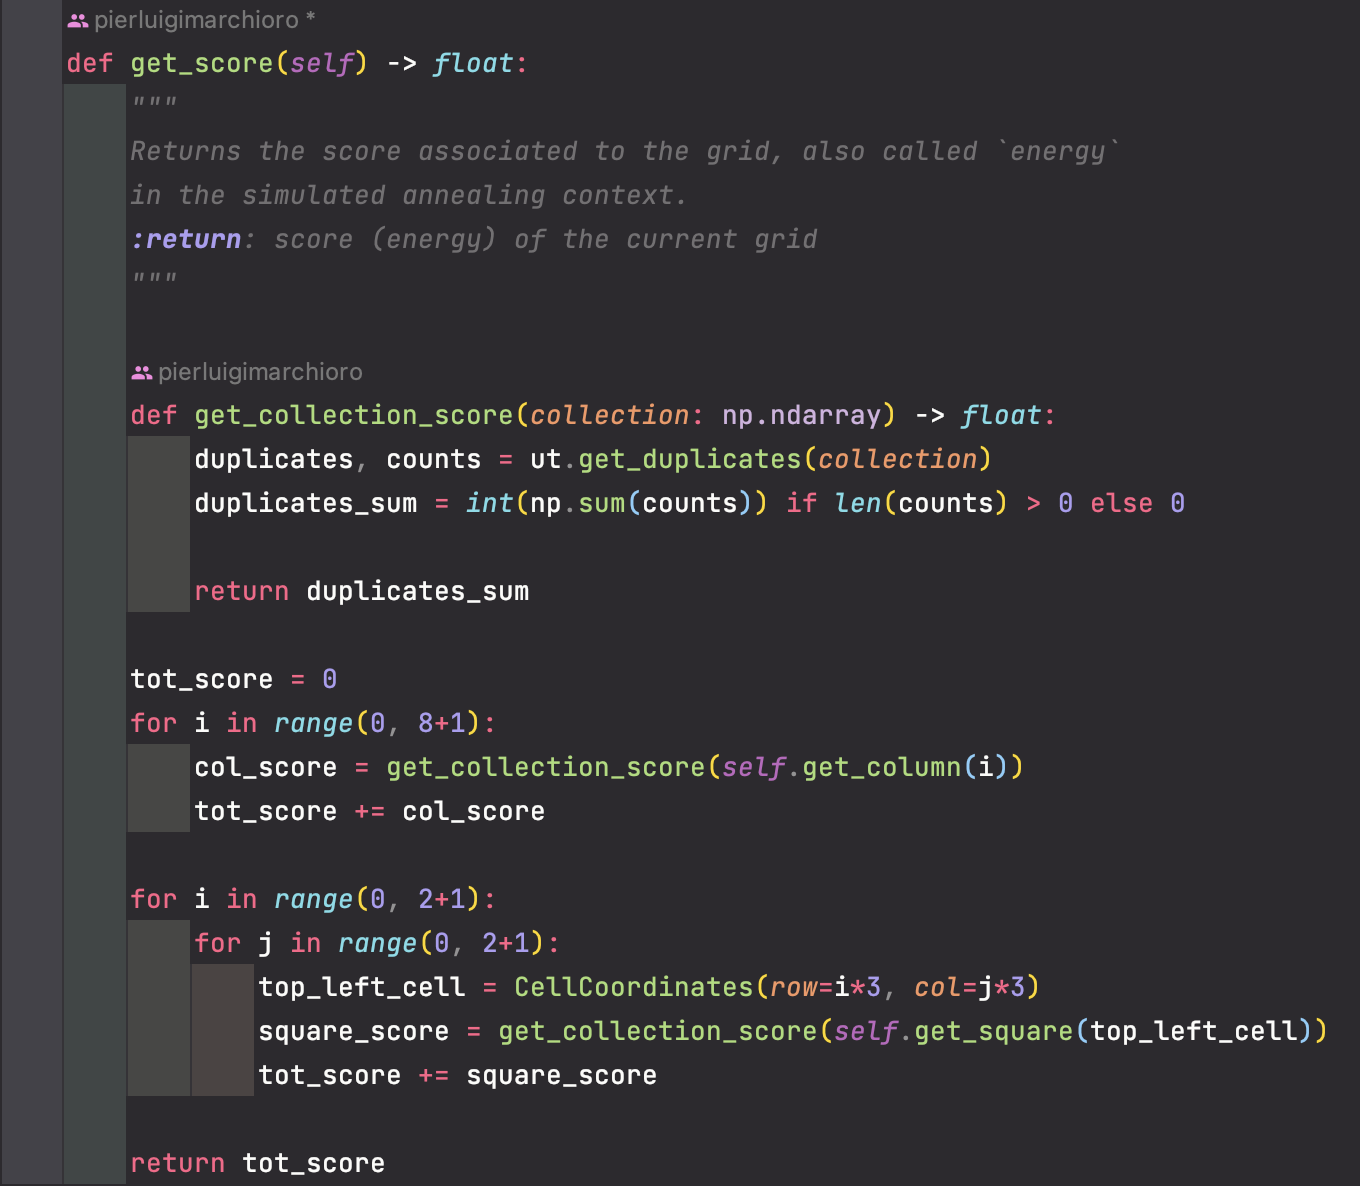
\includegraphics[scale=0.65]{assignment-1/images/sim_ann/energy-1-get_score.png}
    \caption{Implementation of the energy (scoring) function}
    \label{fig:ann_energy_1_get_score}
\end{figure}